\documentclass[12pt]{article}

\usepackage{fullpage}
\usepackage{multicol,multirow}
\usepackage{tabularx}
\usepackage{ulem}
\usepackage[utf8]{inputenc}
\usepackage[russian]{babel}
\textheight=24cm
\usepackage[pdftex]{graphicx}
\graphicspath{{pictures/}}
\DeclareGraphicsExtensions{.pdf,.png,.jpg}

\begin{document}

\section*{Лабораторная работа №\,3 по курсу дискретного анализа: Исследование качества программ}

Выполнил студент группы 08-208 МАИ \textit{Левштанов Денис}.

\subsection*{Условие}

\begin{enumerate}
\item Для реализации словаря из предыдущей лабораторной работы, необходимо провести исследование скорости выполнения и потребления оперативной памяти. В случае выявления ошибок или явных недочётов, требуется их исправить.

\end{enumerate}

\subsection*{Дневник отладки}

\par \textbf{1. gprof}
\par Для проверки своей программы утилитой gprof, я использовал флаг компиляции -pg, затем запускал исполняемый файл с тестами, в результате чего создавался файл gmon.out с данными о времени работы функций программы, затем с помощью самой утилиты gprof, эти данные представляются в понятном виде.
\par Проверив свою программу на 200 000 строк я получил такие результаты: 

\noindent 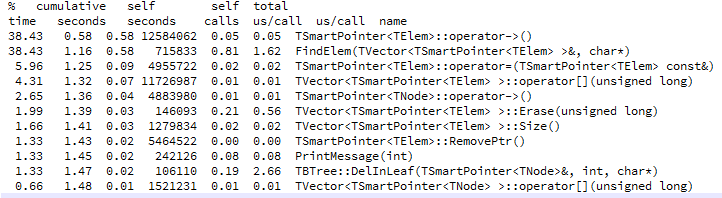
\includegraphics{200k}

Отсюда видно, что намного больше времени, чем все остальные занимают функции operator-> и FindElem. Если operator-> особо ускорить не получится, то функцию FindElem я ускорил, заменив обычный поиск, работающий за O(n), на бинарный, работающий за O(logn). Запустив исправленную программу с этими же тестами я получил:

\noindent 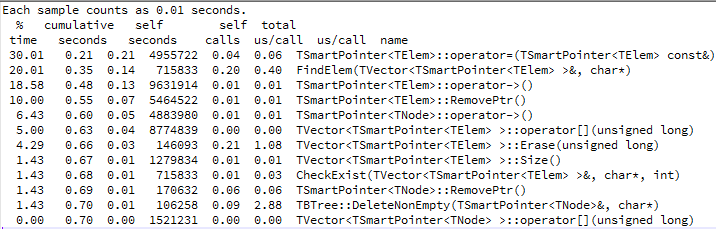
\includegraphics{200kBin}

Тем самым программа ускорилась практически в 4 раза.

\par \textbf{2. valgrind}
\par Valgrind - инстринструментальное программное обеспечение, предназначенное для отладки использования памяти, обнаружения утечек памяти. Запустив свою программму с помощью valgrind --leak-check=full --show-leak-kinds=all, что в некоторых местах не очищается память, тем самым нагружая систему. Для решения этой проблемы и предотвращения ее появления в будущем я написал умные указатели, с помощью которых память освобождается сама.

\noindent 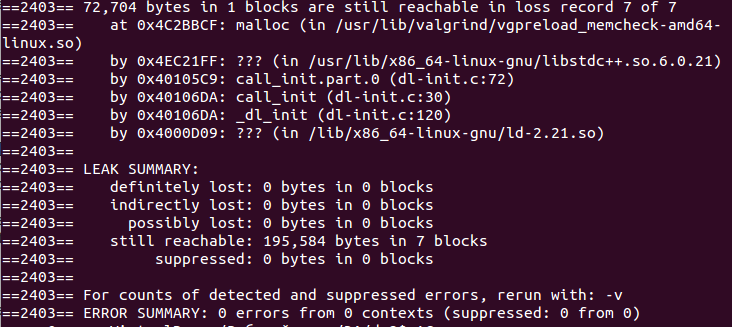
\includegraphics{valgrind}

Также я заметил баг в GCC который теряет 72,704 байт памяти.
\subsection*{Выводы}

Утилита gprof помогает в оптимизации программы, с помощью неё можно узнать функции, в которых она долго работает и локально ее ускорить, не тратя время на ускорение незначительных функций.
Утилита valgrind поможет узнать об утечках памяти, об освобождении уже освобожденной памяти и многие друие ошибки, тем самым не произойдет так, что после долгой работы програмы закончится оперативная память на копьютере.

\end{document}

